\documentclass[t]{myBeamer}


\usepackage{xcolor}
\usepackage[none]{hyphenat} %No hyphenation

\usepackage[utf8]{inputenc}

\usetikzlibrary{calc, positioning, shapes.arrows}
\newcommand\blfootnote[1]{%
  \begingroup
  \renewcommand\thefootnote{}\footnote{#1}%
  \addtocounter{footnote}{-1}%
  \endgroup
}


\usepackage{dirtree}
% The following is a dummy icon command
\newcommand\myicon[1]{{\color{#1}\rule{2ex}{2ex}}}
% If you have actual icon images, use \includegraphics to include them
% If you are generating them, put in the appropriate code for them here
% now we make a command for a folder/file which inserts the icon and its label
% adjust this as needed. If you only have 2 icons, then you could create
% a \myfile and \myfolder command with the icon fixed.
\newcommand{\myfolder}[2]{\myicon{#1}\ {#2}}
\usepackage{listings}


\definecolor{lightGrey}{rgb}{230,230,230}
\definecolor{mygreen}{rgb}{0,0.6,0}
\usepackage{nameref}

\lstset{ %
  backgroundcolor=\color{lightGrey},   % choose the background color; you must add \usepackage{color} or \usepackage{xcolor}; should come as last argument
  basicstyle=\footnotesize,        % the size of the fonts that are used for the code
  breakatwhitespace=true,         % sets if automatic breaks should only happen at whitespace
  breaklines=true,                 % sets automatic line breaking
  commentstyle=\color{mygreen},    % comment style
  frame=single,	                   % adds a frame around the code
  keepspaces=true,                 % keeps spaces in text, useful for keeping indentation of code (possibly needs columns=flexible)
  keywordstyle=\color{blue},       % keyword style
  language=bash,                 % the language of the code  
  showstringspaces=false,
  escapeinside={<@}{@>},
  columns=fullflexible,  
}

\begin{document}
\title{ Fortan Debugging Introduction }   
\author{ \textbf{ Andrés Pérez Hortal} }
\date{April 6, 2018} 

\frame{\titlepage} 



\section{Introduction} 
\subsection{Objectives} 
\begin{frame}[t]
\frametitle{ \huge What is this presentation about? }
  \centering 
  \Large
  \begin{itemize}
    \item Review the \textbf{most common errors} in (Fortran) computer programs    
    \item Present \textbf{simple techniques} to \textbf{find, correct and avoid these errors} in codes.    
  \end{itemize}
\end{frame}

\subsection{Definitions} 
\begin{frame}[t]
\frametitle{ \huge What is a computer error or ``bug''?}
  \centering 
  
  \Large
  
  \begin{itemize}
  \setlength\itemsep{0ex}
  \setlength\parsep{0pt}
  \setlength\parskip{0pt}
   
    \item \makebox[3cm][l]{\textbf{Software bug}} : An error, flaw, failure or fault in a computer program or system that causes it to produce an incorrect or unexpected result, or to behave in unintended ways.
    \vspace{10pt}
    
    \end{itemize}

\end{frame}

\begin{frame}[t]
\frametitle{ \huge Why ``bug''?}
  \centering 
  
  \Large
  
  \begin{itemize}
  \setlength\itemsep{0ex}
  \setlength\parsep{0pt}
  \setlength\parskip{0pt}
   
    \item \textbf{Popular attribution}: In 1946, Grace Hopper traced an error in the Mark II to a moth trapped in a relay, a ``bug''.
    \item \textbf{First use} dates back to Thomas Edison in 1876 to refer to the failures in his experiments. 
  
    \end{itemize} 

\end{frame}



\begin{frame}[t]
\frametitle{ \huge What is debugging?}
  \centering 
  \Large  
  \begin{itemize}
    \item The process of \textbf{finding and resolving} defects or problems within the program that prevent correct operation of computer software.
    \item Debugging is not only about finding and solving problems with your code. It is also increasing your understanding of how the code works.
    \end{itemize}

\end{frame}

\section{Types of errors} 
\begin{frame}[t]
\frametitle{ \huge Types of errors }
  
  
  \begin{tightBox}
  \centering 
  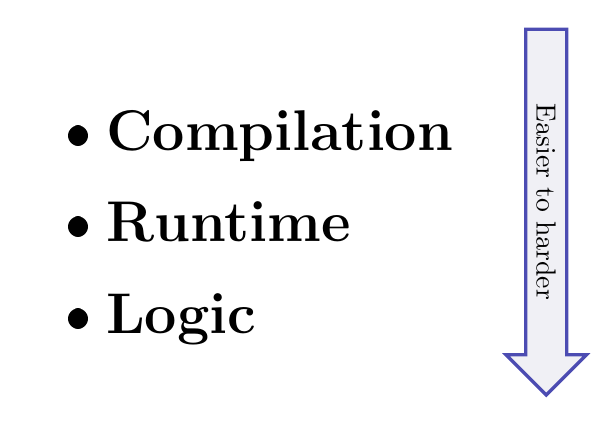
\begin{tikzpicture}[node distance=0pt,
		      SA/.style = {single arrow, draw=blue!40!gray, very thick, fill=blue!20!gray!10,
		      minimum height=1.2*\n1} ]
		      
   \node (n)   [text width=0.5\textwidth]
{
  \huge
      \begin{itemize}	
	\item \textbf{Compilation}
	\item \textbf{Runtime}
	\item \textbf{Logic}
      \end{itemize}    
};
\path   let \p1 = ($(n.north)-(n.south)$),
            \n1 = {veclen(\y1,\x1)} in
        node[SA, rotate=-90,  xshift=-\n1/2,
             above=of n.south east] {Easier to harder};
\end{tikzpicture}
  \end{tightBox}
\end{frame}  



\subsubsection{Compilation errors} 
\begin{frame}[t]
\frametitle{ \huge Compilation errors }
\Large
\begin{itemize}
  \item Errors that appears during the compilation process (translating code to machine language)  
  \item Detected and pointed out by the compiler.  
  \item The line number in the source code where the problem is located is typically indicated by the compiler.
\end{itemize}
\end{frame}

\subsubsection{Runtime errors} 

\begin{frame}[t]
\frametitle{ \huge Runtime errors}
\Large
\begin{itemize}
  \item Error that occurs when you run your program
  \item The failure is a result of an error that propagates and produce a failure in the program.
  \item Some of them can be prevent by the compiler! More on compiler warnings coming next.
  \item Difficult to solve
  \item E.g.: Memory leaks, segmentation fault, infinity loops, more segmentation faults...
\end{itemize}
\end{frame}

\subsubsection{Logical errors} 
\begin{frame}[t]
\frametitle{ \huge Logical errors}
\Large
\begin{itemize}
  \item The program appears to run correctly, by it gives wrong or unexpected results
  \item Most difficult to correct
  \item One approach to solve them is to test different parts of the program with inputs with known outputs.
\end{itemize}
\end{frame}


\setbeamercolor{alerted text}{fg=black,bg=}

\section{Compilation errors} 

\begin{frame}[t]
\frametitle{ \huge Types of errors }
  
  \setbeamercovered{transparent}
  \begin{tightBox}
  \centering 
  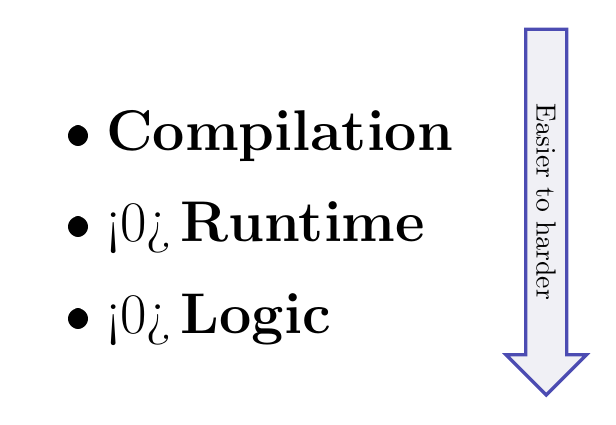
\begin{tikzpicture}[node distance=0pt,
		      SA/.style = {single arrow, draw=blue!40!gray, very thick, fill=blue!20!gray!10,
		      minimum height=1.2*\n1} ]
		      
   \node (n)   [text width=0.5\textwidth]
{
  \huge
      \begin{itemize}	
	\item \textbf{Compilation}
	\item<0> \textbf{Runtime}
	\item<0> \textbf{Logic}
      \end{itemize}           
};
\path   let \p1 = ($(n.north)-(n.south)$),
            \n1 = {veclen(\y1,\x1)} in
        node[SA, rotate=-90,  xshift=-\n1/2,
             above=of n.south east] {Easier to harder};
\end{tikzpicture}
  \end{tightBox}
 
\end{frame}  

\subsection{Compilation process} 
\begin{frame}[t]
\frametitle{ \huge Understanding the compilation process}
\centering
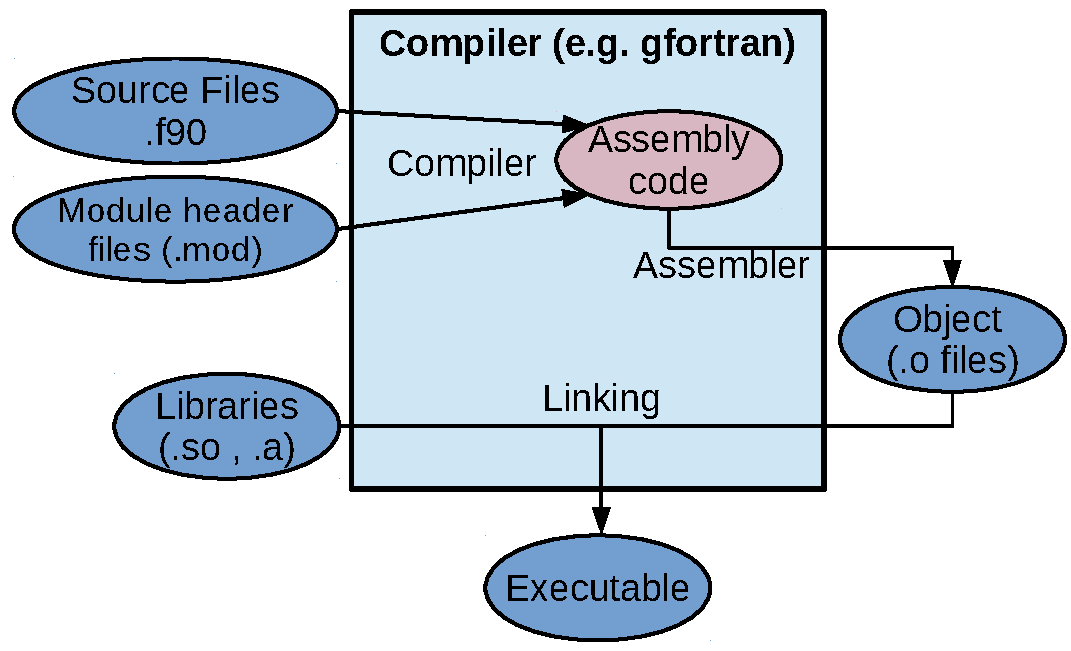
\includegraphics[height=0.7\textheight]{img/compilationProcess.pdf} 
\end{frame}



\begin{frame}[t]
\frametitle{ \huge Differences between header and sources}
\begin{itemize}
 \item The dependency structure in Fortran 90 is somewhat complex and compiler-dependent.
 \item The basic model is like C with source (.f90)  and header (.mod) files.
 \item The \textbf{source} codes defines the \textbf{functions, subroutine or the main program}. 
 \item The \textbf{header} (.mod) files specify \textbf{interfaces, derived types, and similar information}.
 \item \textbf{The header is the interface to whatever is implemented in the corresponding sources (.f90) files.}  
\end{itemize}
\end{frame}

\begin{frame}[t]
\frametitle{ \huge What is an object?}

\only<+>{\centering 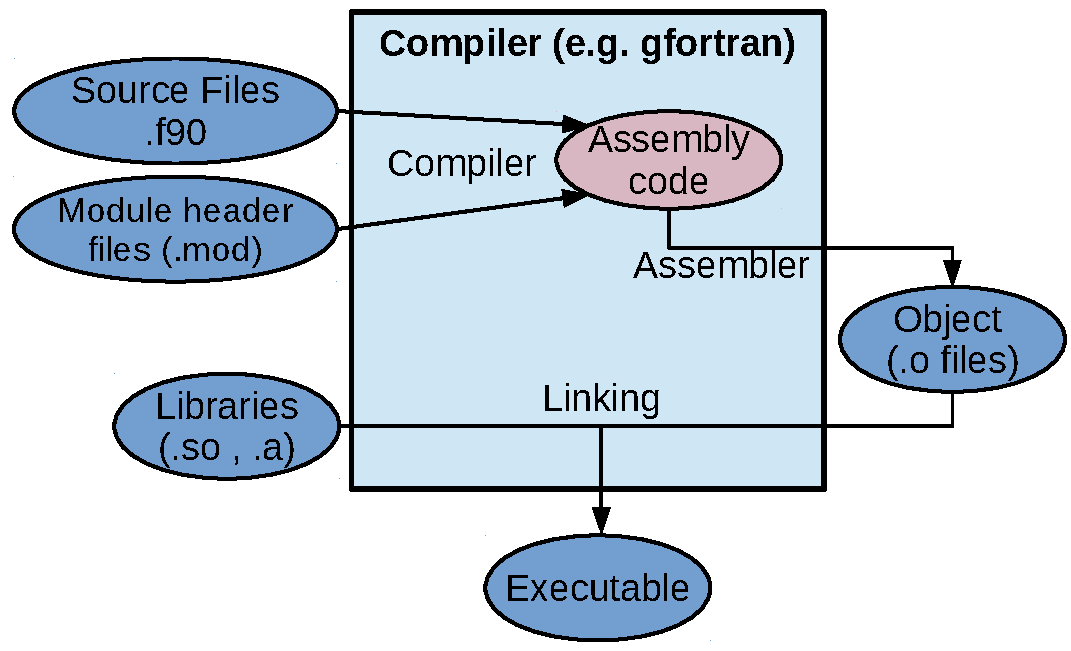
\includegraphics[height=0.7\textheight]{img/compilationProcess.pdf} }
\only<+>{
\large
\begin{itemize}
 \item Each source file is translated (compiled) separately by the compiler into an object (.o) file. 
 \item Provides external symbols that can be used by other objects and libraries (exports).
 \item List of symbols expected from other objects and libraries (imports) . 
\end{itemize}
}
\end{frame}



\begin{frame}[fragile]
\frametitle{ \Large Source example:simple\_module.90 }
\footnotesize

\begin{lstlisting}[language=fortran]
MODULE simple_module
  IMPLICIT NONE
    PRIVATE multiply
  CONTAINS
    
    REAL FUNCTION multiply(a, b) !Visible inside the module (PRIVATE)
      REAL, INTENT(IN) :: a, b
      multiply = a*b
    END FUNCTION   
    !volume is visible from outside the module (PUBLIC)
    REAL FUNCTION volume(width, height, depth) 
      REAL :: rectagle_area !external function!
      REAL, INTENT(IN) :: width, height, depth
      REAL :: my_area	  
      my_area = rectagle_area(width ,height )
      volume = multiply(my_area, depth)
    END FUNCTION
END MODULE simple_module
\end{lstlisting}


\end{frame}

\begin{frame}[fragile,t]
\frametitle{ \Large Object example: simple\_module.o}
\footnotesize

\begin{lstlisting}[language=bash]
$ gfortran -c simple_module.f90 # Compile source
$ nm simple_module.o # Object viewer
                         U rectagle_area_                      #"U" undefined symbol
0000000000000062 t __simple_module_MOD_multiply #"t" internal symbol 
0000000000000000 T __simple_module_MOD_volume #"T" external symbol
\end{lstlisting}


\begin{tightBox}
\centering \Large
\textbf{Symbols}: variables, functions, or subroutines
\end{tightBox}

\begin{tightBox}
\centering \Large
\textbf{Important}: Remember that the objects may have undefined symbols!!
\\
\large We are going to come back to this later.
\end{tightBox}

\end{frame}


%https://stackoverflow.com/questions/12237282/whats-the-difference-between-so-la-and-a-library-files
\begin{frame}[t]
\frametitle{ \huge What is a library?}
\large
\begin{itemize}
 \item A collection of object files. Just a bunch of object files glued together.
 \item Files are built from compiled object files (.o files)
 \item \textbf{Static libraries} (.a files): Archives of objects. Objects are copied to the executable during linking.
 \item \textbf{Dynamic libraries} (.so files): The suffix stands for "shared object".
 All the applications that are linked with the library use the same file
 rather than making a copy in the resulting executable.
\end{itemize}
\end{frame}

\subsubsection{Linking} 
\begin{frame}[t]
\frametitle{ \huge What is linking process?}

\large
\begin{itemize}
 \item Combines one or more object files into a single executable file, library file, or another 'object' file.
\end{itemize}

\centering
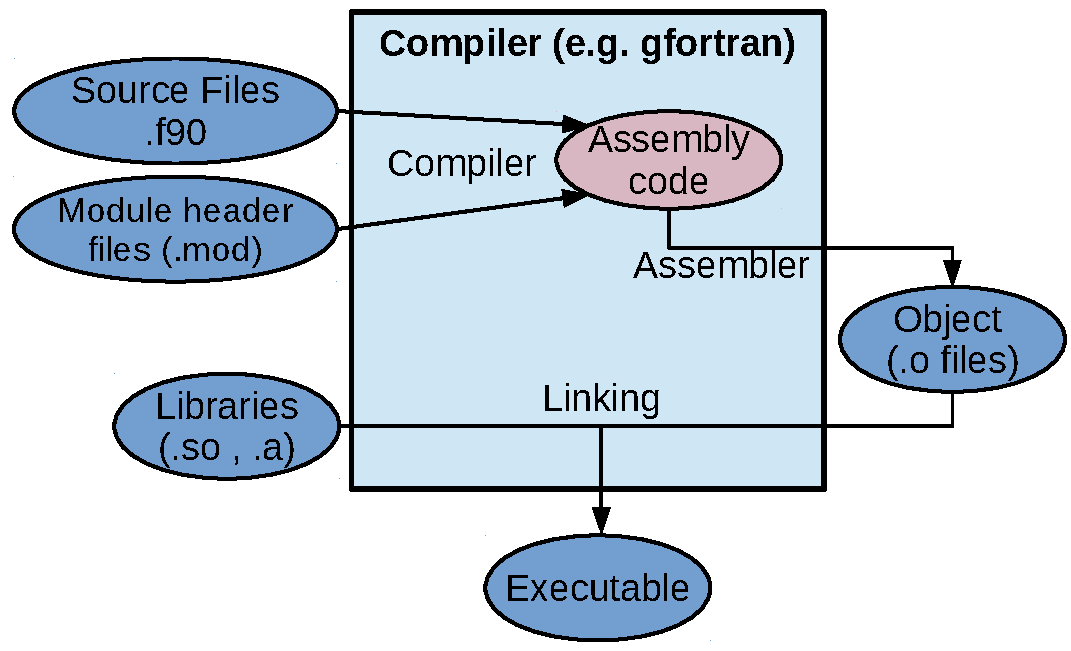
\includegraphics[height=0.5\textheight]{img/compilationProcess.pdf} 
\end{frame}


\subsubsection{Compilation example} 

\begin{frame}[t]
\frametitle{ \huge Program compilation example 1}

\only<+>{
\begin{tcolorbox}[colback=mcgillred!5,
  colframe=mcgillred,boxsep=2pt,
  left=0pt,right=0pt,top=5pt,bottom=5pt, title=\textbf{Program that use an external module}]
  
  \begin{columns}
  \begin{column}{0.6\textwidth}
\dirtree{%
.1 \myfolder{blue}{example\_project}.
.2 \myfolder{green}{myProgram.f90}.
.2 \myfolder{blue}{externalModule}.
.3 \myfolder{green}{externalModule.f90}.
}
\end{column}

  \begin{column}{0.4\textwidth}
    \textbf{myProgram} calls a function in \textbf{externalModule}
  \end{column}
\end{columns}

\end{tcolorbox}

\begin{tcolorbox}[colback=blue!5,
  colframe=blue,boxsep=1pt,
  left=0pt,right=0pt,top=5pt,bottom=5pt, title=\textbf{Compilation steps}]
\begin{itemize}
 \item Compile \textbf{externalModule.f90} ( .o and .mod files)
 \item Compile  \textbf{myProgram.f90} ( .o )
 \item Link \textbf{myProgram} with \textbf{externalModule}
\end{itemize}
\end{tcolorbox}
}
\end{frame}

\begin{frame}[fragile]
\frametitle{ \huge Program compilation example 1 }
\vspace{-15pt}
\footnotesize
\begin{lstlisting}[language=bash]
### Compilation Procedure ###

# Compile the external module (no linking!)
cd externalModule # Change directory
#   -c : Compile to an object file
#   -o : Specifies the name of the output file.
gfortran -c externalModule.f90 -o externalModule.o

# Compile the myProgram.f90 program (no linking!)
cd .. # Return to the project dir
#  -I : adds include directory of header (.mod) files 
gfortran -I./externalModule -c myProgram.f90 -o myProgram.o

# Link myProgram and the external module to create the executable
gfortran myProgram.o externalModule/externalModule.o -o myProgram
\end{lstlisting}

\end{frame}



\begin{frame}[t]
\frametitle{ \huge Program compilation example 2}

\only<+>{
\begin{tcolorbox}[colback=mcgillred!5,
  colframe=mcgillred,boxsep=2pt,
  left=0pt,right=0pt,top=5pt,bottom=5pt, title=\textbf{Program that use an external library}]
  
  \begin{columns}
  \begin{column}{0.65\textwidth}
\dirtree{%
.1 \myfolder{blue}{example\_project\_2}.
.2 \myfolder{green}{myProgram.f90}.
.2 \myfolder{blue}{myLibrary}.
.3 \myfolder{blue}{src}.
.4 \myfolder{green}{module\_circle.f90}.
.4 \myfolder{green}{module\_rectangle.f90}.
.3 \myfolder{blue}{lib}.
.4 \myfolder{green}{libgeometry.a}.
.3 \myfolder{blue}{include}.
.4 \myfolder{green}{myLibrary.mod}.
}
\end{column}

  \begin{column}{0.35\textwidth}
    \textbf{myProgram} calls a function \\
    in \textbf{the library libgeometry.a}
  \end{column}
\end{columns}

\end{tcolorbox}

}
\end{frame}

\begin{frame}[fragile]
\frametitle{ \huge Program compilation example 2}
\footnotesize
\vspace{-15pt}
\begin{lstlisting}[language=bash]
### Compilation Procedure ###
# Compile the library first
cd myLibrary # Change directory
#  -J : This option specifies where to put .mod files.
gfortran -Jinclude  -c module_circle.f90 -o module_circle.o
gfortran -Jinclude  -c module_rectangle.f90 -o module_rectangle.o

# Now let's create my static library "libgeometry"
ar -rv lib/libgeometry.a module_circle.o module_rectangle.o

# Compile the myProgram.f90 program (no linking!)
cd .. # Return to the project dir
gfortran  -I./myLibrary/include -c myProgram.f90

# Link myProgram and the external module to create the executable
# -lName : Search the library named "libName.a" or "libName.so"
# -L: Add directories where libraries are search
gfortran myProgram.o -L./myLibrary/lib -lgeometry -o myProgram
\end{lstlisting}

\end{frame}


\subsection{Types} 

\begin{frame}[t]
\frametitle{ \huge Back to the compilation errors...}
\Huge
  \begin{center}
    \begin{minipage}{0.6\textwidth}
      \begin{tightBox}
	  \begin{itemize}
	    \item Syntax
	    \item Type mismatch
	    \item Linking
	  \end{itemize}
      \end{tightBox}
    \end{minipage}
    \end{center}
\end{frame}

 
\subsection{Syntax} 
\begin{frame}[t]

\frametitle{ \huge Compilation errors: \textbf{Syntax} }
\Large
\only<1>{
\begin{itemize}
  \item Error in the syntax of a sequence of characters or tokens that is intended to be written in a particular programming language.
\end{itemize}
}
\only<2>{ \centering 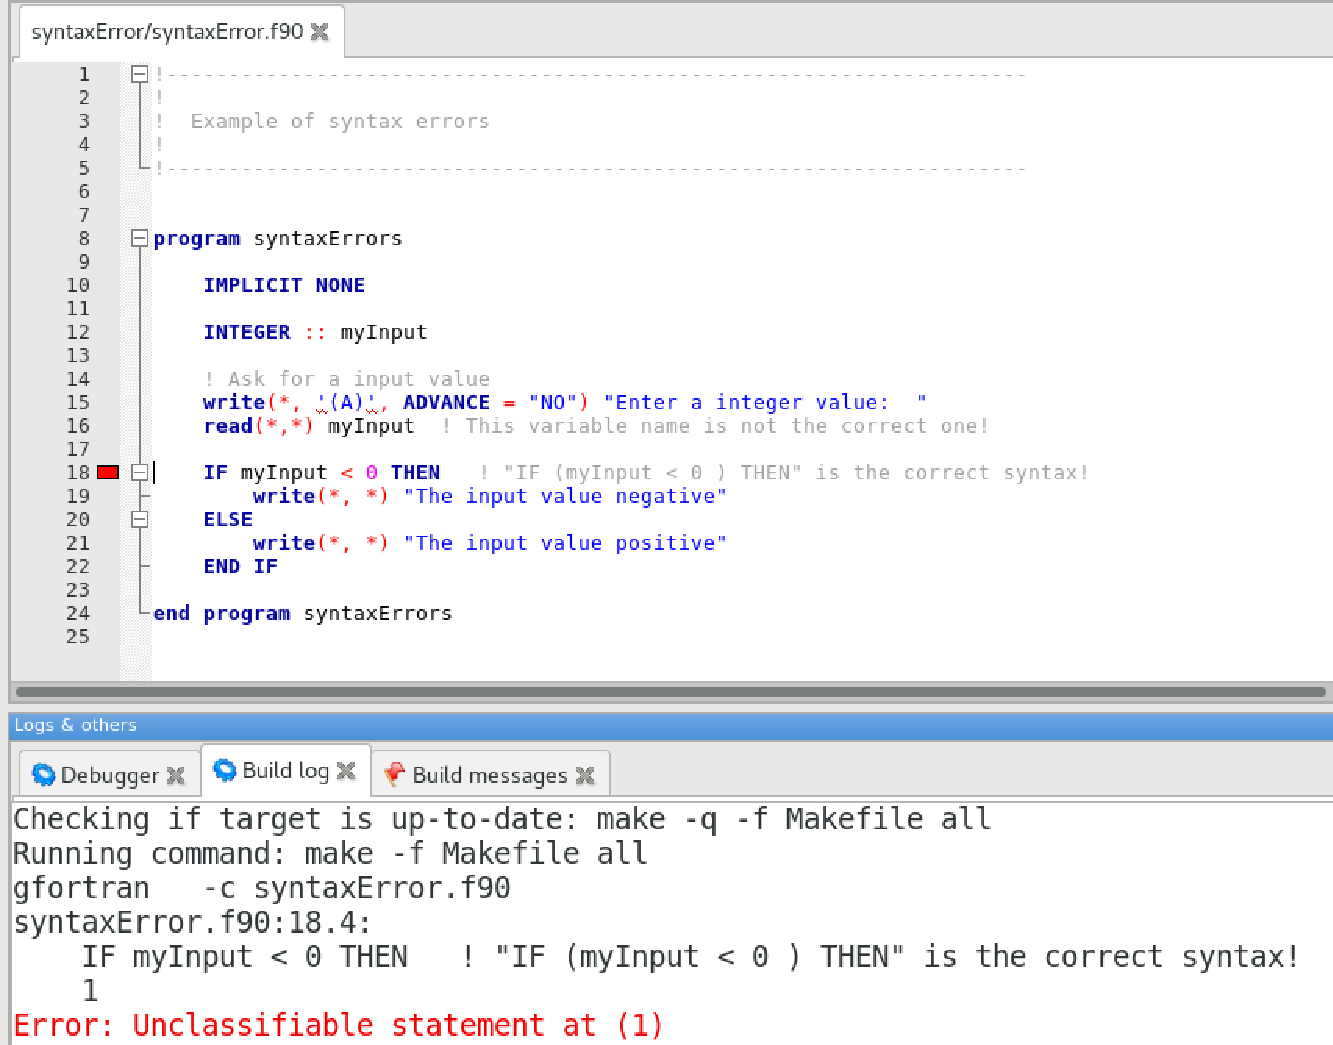
\includegraphics[height=0.7\textheight]{img/syntaxError.pdf} }

\end{frame}


\subsection{Type mismatch} 
\begin{frame}[t]

\frametitle{ Compilation errors: \textbf{Type mismatch} }
\Large
\only<1>{ 
\begin{itemize}
  \item Calling a function or procedure with arguments that are not the expected ones.
\end{itemize}
}

\only<2>{ \centering 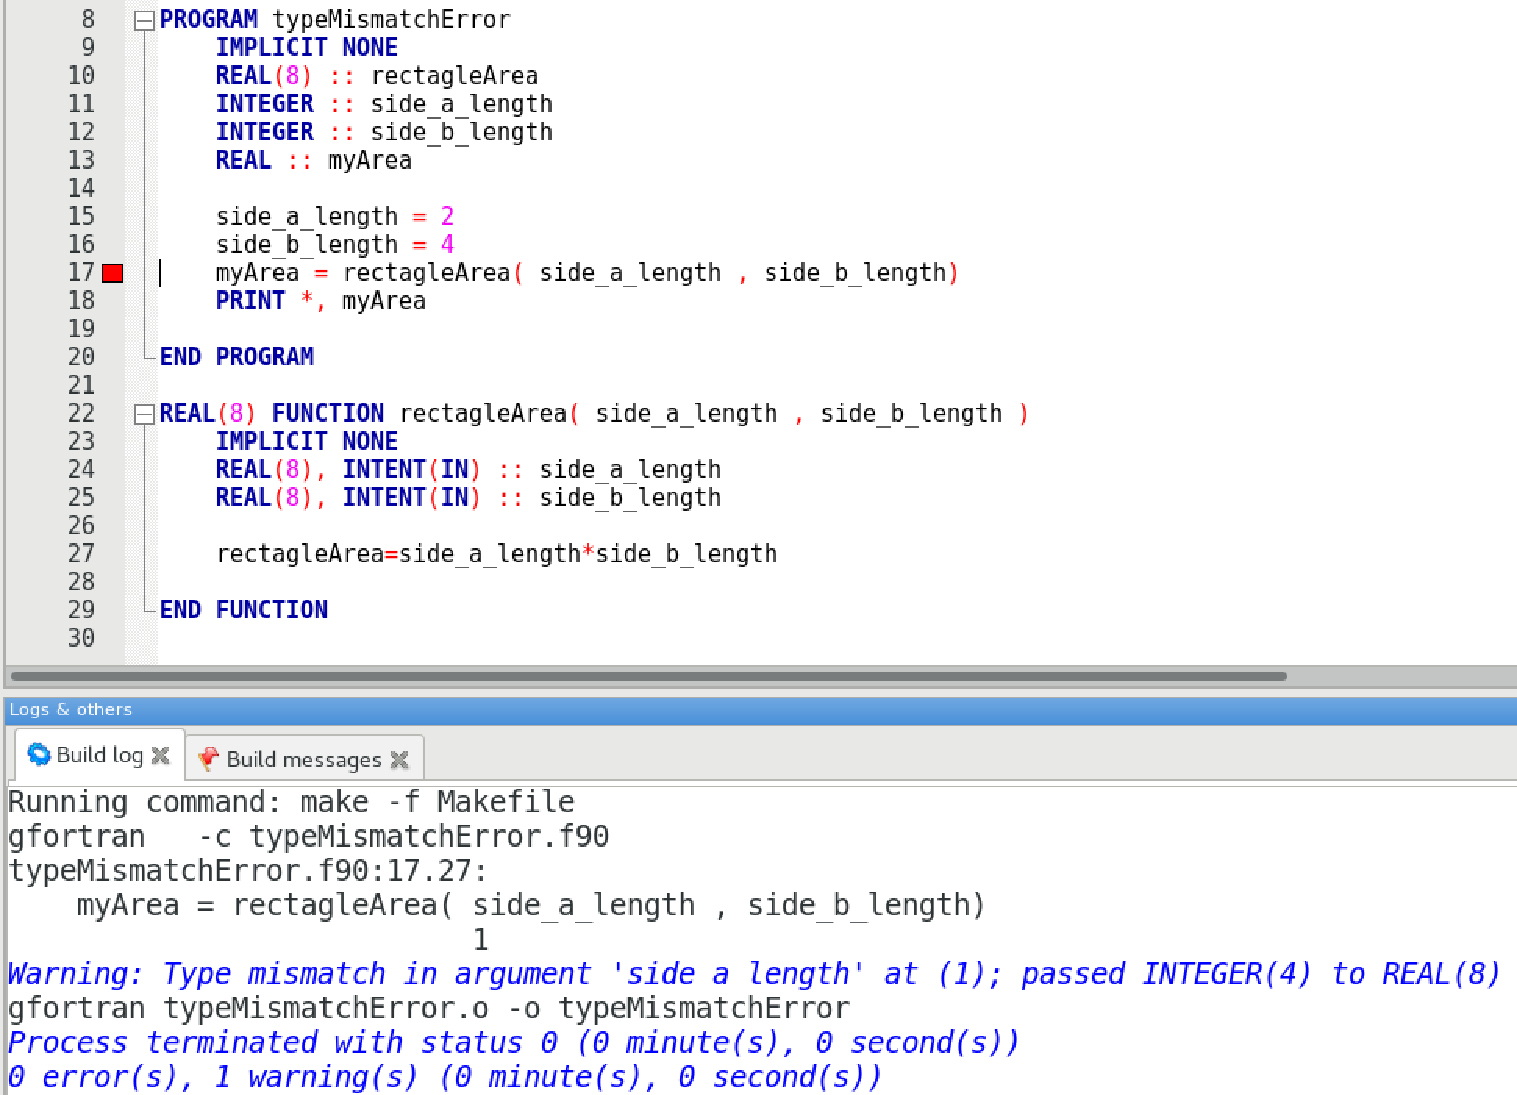
\includegraphics[height=0.7\textheight]{img/typeMismatchError.pdf} }

\end{frame}

\subsection{Linking} 
\begin{frame}[t]
%TODO: Debugging example: add the -llib before the target!!!
%TODO: Use ld -LmyLibrary/lib -lmyLibrary --verbose to see if the library is found
%TODO: Then change order
\frametitle{ \huge Compilation errors: \textbf{Linking} }
\Large
\only<1>{ 
\begin{itemize}
  \item The source code is compiled successfully, but the objects can be linked
  \item E.g. missing library or function
\end{itemize}

% % \begin{tightBox}
% % \begin{center}
% % \textbf{This why we review the Compilation Procedure!} 
% % \end{center}
% % \end{tightBox}

}

% \only<2>{ \centering 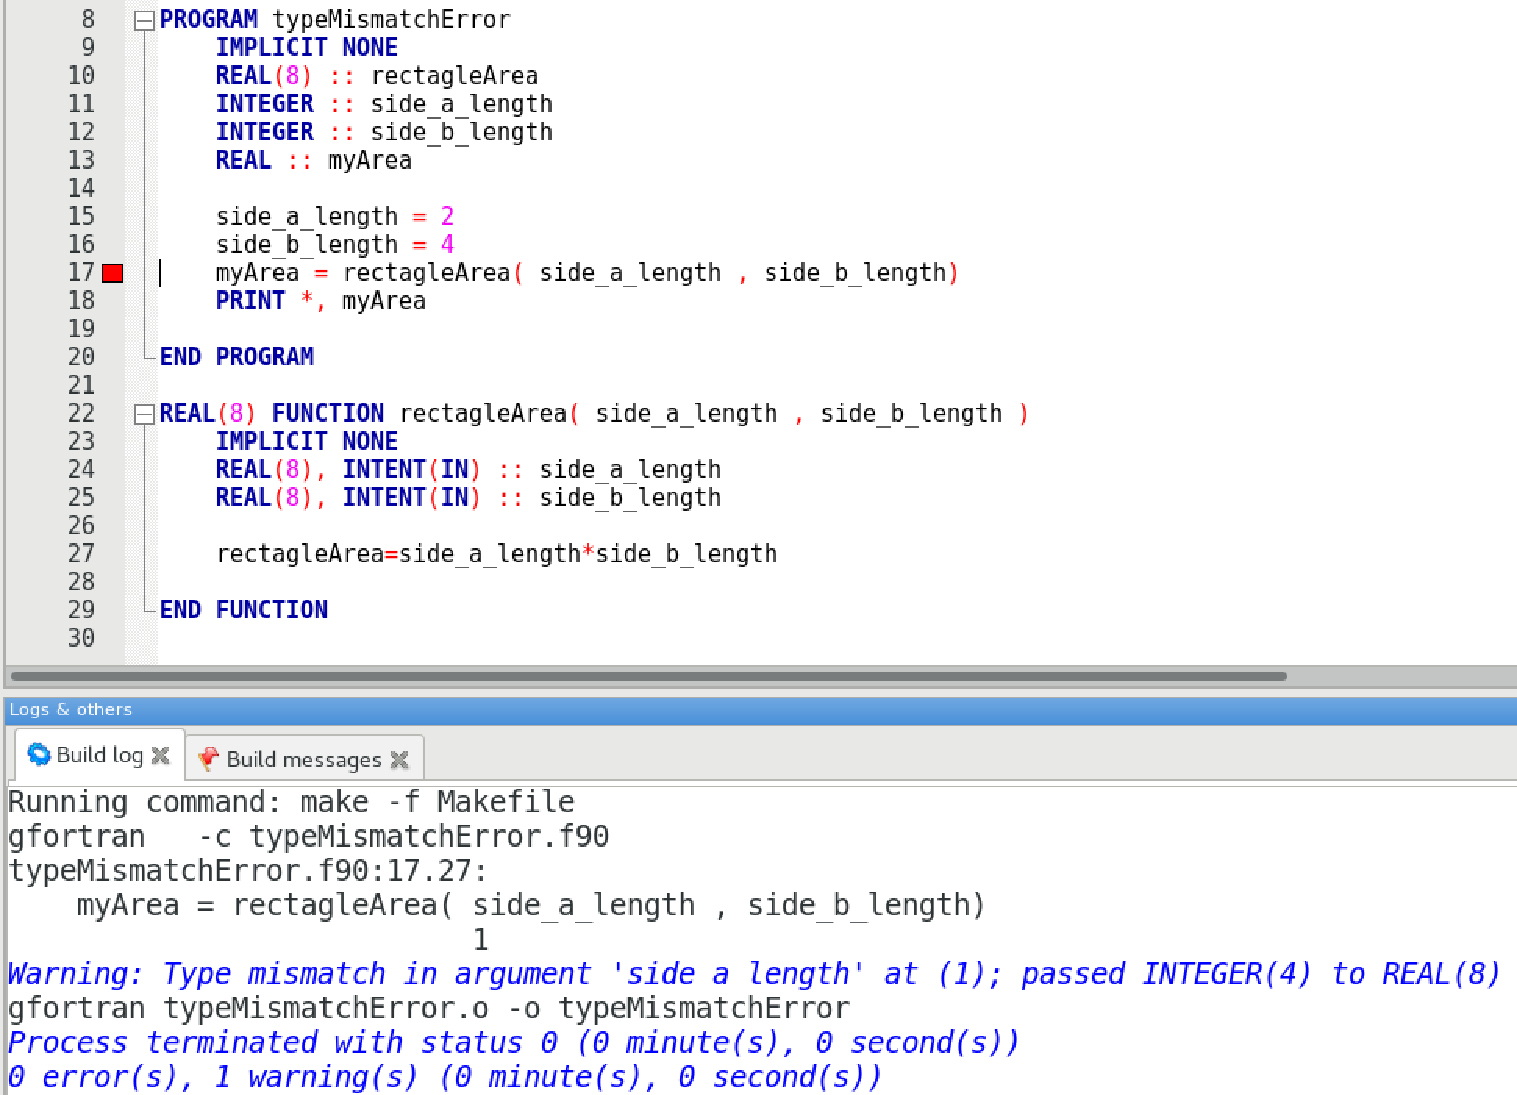
\includegraphics[height=0.7\textheight]{img/typeMismatchError.pdf} }
% \only<3>{ \centering 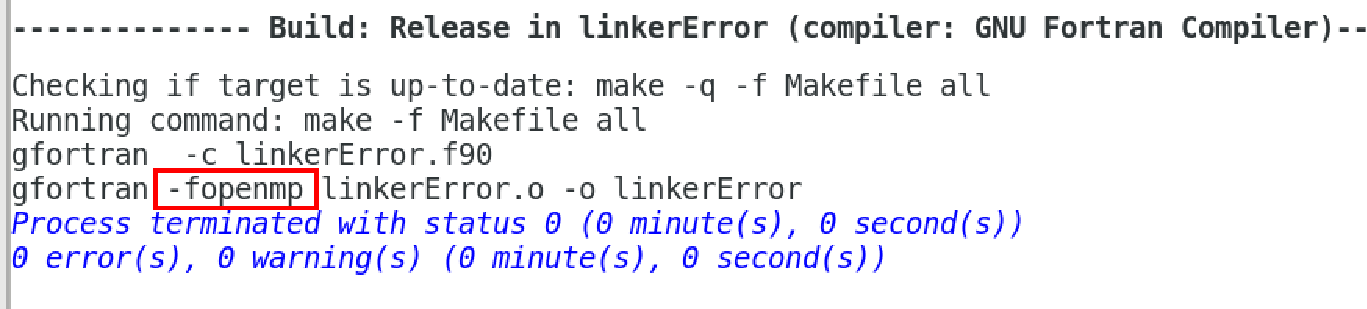
\includegraphics[width=\textwidth]{img/LinkerError_Solved.pdf} }

\end{frame}


\begin{frame}[t]
\frametitle{ \huge Program compilation example 2}

\only<+>{
\begin{tcolorbox}[colback=mcgillred!5,
  colframe=mcgillred,boxsep=2pt,
  left=0pt,right=0pt,top=5pt,bottom=5pt, title=\textbf{Program that use an external library}]
  
  \begin{columns}
  \begin{column}{0.65\textwidth}
\dirtree{%
.1 \myfolder{blue}{example\_project\_2}.
.2 \myfolder{green}{myProgram.f90}.
.2 \myfolder{blue}{myLibrary}.
.3 \myfolder{blue}{src}.
.4 \myfolder{green}{module\_circle.f90}.
.4 \myfolder{green}{module\_rectangle.f90}.
.3 \myfolder{blue}{lib}.
.4 \myfolder{green}{libgeometry.a}.
.3 \myfolder{blue}{include}.
.4 \myfolder{green}{myLibrary.mod}.
}
\end{column}

  \begin{column}{0.35\textwidth}
    \textbf{myProgram} calls a function \\
    in \textbf{the library libgeometry.a}
  \end{column}
\end{columns}

\end{tcolorbox}

}
\end{frame}

\begin{frame}[fragile, t]
\frametitle{ \huge Example project: Compilation commands }
\footnotesize
\vspace{-12pt}
\begin{lstlisting}[language=bash]
# ERROR DURING LINKING
# Object that needs the library was placed after the libraries definitions.

# Link myProgram and the external module to create the executable
# -lName : Search the library named "libName.a" or "libName.so"
# -L: Add directories where libraries are search
$ gfortran -L./myLibrary/lib -lgeometry myProgram.o  -o myProgram

myProgram.o: In function `MAIN__':
myProgram.f90:(.text+0x4e): undefined reference to
  `__module_rectangle_MOD_rectagle_area'
collect2: error: ld returned 1 exit status
\end{lstlisting}
\begin{tightBox}
 \centering \huge \textbf{Why did this happen?}
\end{tightBox}


%TODO: Use ld -LmyLibrary/lib -lmyLibrary --verbose to see if the library is found
%TODO: Then change order
\end{frame}



\begin{frame}[t]
\frametitle{ \Large Lets review the linking process...
\footnote{https://eli.thegreenplace.net/2013/07/09/library-order-in-static-linking}}

\Large

\only<+>{
\begin{itemize}
 \item{The linker maintains a symbol table with two lists: 
  \begin{itemize}\Large    
    \item A list of \textbf{symbols exported} by all the objects and libraries encountered so far.
    \item A list of \textbf{undefined symbols} that the encountered objects and libraries requested to import and were not found yet. 
  \end{itemize}
  }
\end{itemize} 
}

\only<+>{
  \begin{itemize}
  \item{When the linker encounters a new object file, it looks at:
  \begin{itemize}\Large   
       \item The \textbf{symbols it exports}: these are added to the list of exported symbols. If any symbol is in the undefined list, it's removed from there because it has now been found.
       \item The \textbf{symbols it imports}: these are added to the list of undefined symbols, unless they can be found in the list of exported symbols.
   \end{itemize}
   }
   \end{itemize} 
}

\only<+>{
   \begin{itemize}
   \item{When the linker encounters a new library.   
   \begin{itemize}
      \item The linker goes over all the objects in the library. 
      \item Add \textbf{only} the objects that contain symbols that are on the undefined list.      
    \end{itemize}
    }
    \item{When the linker finishes
    \begin{itemize}
      \item If any symbols remain in the undefined list, the linker throw an \textbf{``undefined reference'' error}.
      \item Note that after the linker has looked at a library, it won't look at it again.
    \end{itemize}}
    \end{itemize} 
}    
    
\end{frame}

\begin{frame}[fragile, t]
\frametitle{ \huge Back to the linking error... }
\footnotesize
\vspace{-12pt}
\begin{lstlisting}[language=bash]
# ERROR DURING LINKING
# Object that needs the library was placed after the libraries definitions.

# Link myProgram and the external module to create the executable
# -lName : Search the library named "libName.a" or "libName.so"
# -L: Add directories where libraries are search
$ gfortran -L./myLibrary/lib -lgeometry myProgram.o  -o myProgram

myProgram.o: In function `MAIN__':
myProgram.f90:(.text+0x4e): undefined reference to
  `__module_rectangle_MOD_rectagle_area'
collect2: error: ld returned 1 exit status
\end{lstlisting}
\begin{tightBox}
 \centering \huge \textbf{Why did this happen?}
\end{tightBox}


%TODO: Use ld -LmyLibrary/lib -lmyLibrary --verbose to see if the library is found
%TODO: Then change order
\end{frame}


% %TODO: Use ld -LmyLibrary/lib -lmyLibrary --verbose to see if the library is found
% %TODO: Then change order





% Runtime errors: memory leaks, ifinite loops, 

% Debbugging techniques 
%  ** (runtime)****
%  * Print debugging (tracing)
%  * Analisis of the stacktraces , what is the stack?? Example of runtime errors...
%  * Narrow dow the portion of the running program until the error is found
%  * Use debugging tools (like gdb, or IDE)
% Part 3: Changing things
%  Every change, o matter how small it is , can introduce a bug. 
%  The obvious thing is start changing things to see what is wrong... This is a very bad idea... You can end braking he system. Ding more harm than good.
%  Add debuggin information...

% Part 4: Preventive measures
% Introduce small changes and then test the code. If something fail, it is easier to track the probelm


\section{Runtime errors} 

\begin{frame}[t]
\frametitle{ \huge Runtime errors }
  \Large
  \setbeamercovered{transparent}
  \begin{tightBox}
  \centering 
  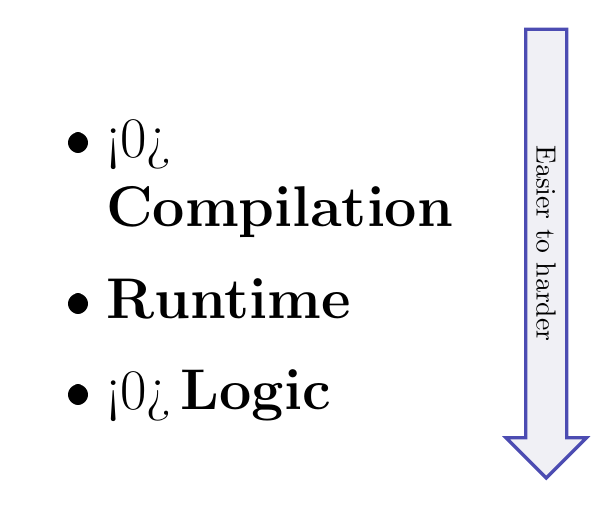
\begin{tikzpicture}[node distance=0pt,
		      SA/.style = {single arrow, draw=blue!40!gray, very thick, fill=blue!20!gray!10,
		      minimum height=1.2*\n1} ]
		      
   \node (n)   [text width=0.5\textwidth]
{
  \huge
      \begin{itemize}	
	\item<0> \textbf{Compilation}
	\item \textbf{Runtime}
	\item<0> \textbf{Logic}
      \end{itemize}           
};
\path   let \p1 = ($(n.north)-(n.south)$),
            \n1 = {veclen(\y1,\x1)} in
        node[SA, rotate=-90,  xshift=-\n1/2,
             above=of n.south east] {Easier to harder};
\end{tikzpicture}
  \end{tightBox}
 
\end{frame}  


\begin{frame}[t]
\frametitle{ \huge Common Runtime errors }
  \Large
      \begin{itemize}	
	\item Segmentation fault
	\item Infinity loops
	\item Uninitialized variables
	\item Arithmetic operations errors	
      \end{itemize}       
\end{frame}  


\subsection{Segmentation fault} 
\begin{frame}[t]
\frametitle{ \huge Segmentation fault }
\Large
\only<+>{
      \begin{itemize}	
	\item Specific kind of error caused by accessing memory that ``does not belong to you.'' 
	\item It is a helper mechanism that keeps you from corrupting the memory and introducing hard-to-debug memory bugs.
	\item{It can happen when:
	  \begin{itemize}
	  \item Accessing variable that has already been freed
	  \item Writing to a read-only portion of the memory
	  \item Accessing an indexes of an arrays that is beyond its dimension
	  \end{itemize}  
	  }
      \end{itemize}     
}
\only<+>{
\begin{itemize}	
      \item{Contrary to other languages, Fortran is not able to properly handle invalid
      memory access on runtime.}
      \item{If an index is out of scope, Fortran
      will not see it and a memory corruption might appear.}
      \end{itemize} 
}
\end{frame}  


\subsection{Segmentation fault example} 
\subsubsection{Code} 
\begin{frame}[fragile,t]
\frametitle{ \huge Segmentation fault example: Code}
\vspace{-10pt}
\begin{lstlisting}[language=fortran,numbers=left]
program segmentation_fault
implicit none
integer :: i

real,dimension(4) :: one_array
write(*,*) "one_array elements: From",loc(one_array),"to",loc(one_array)+4*9
write(*,*) "i location relative to one_array(0):", loc(i)-loc(one_array)
write(*,*)

write(*,*) '                              index          memory address'
do i = 1,10
    write(*,*) 'Writing "10" for index',i, "  at",loc(one_array(i))-loc(one_array)
    one_array(i)=10
enddo
end program
\end{lstlisting}

\end{frame}  

\subsubsection{Output} 
\begin{frame}[fragile,t]
\frametitle{ \huge Segmentation fault example: Output}
\vspace{-10pt}
\begin{lstlisting}[language=bash]
 one_array elements: From      140735594477648 to      140735594477684
 i location relative to one_array(0):                   28

                                     index           memory address
 Writing "10" for index           1     at                    0
 Writing "10" for index           2     at                    4
 Writing "10" for index           3     at                    8
 Writing "10" for index           4     at                   12 #one_array(4)
 Writing "10" for index           5     at                   16 #???
 Writing "10" for index           6     at                   20 #???
 Writing "10" for index           7     at                   24 #???
 Writing "10" for index           8     at                   28 # "i"
 Writing "10" for index  1092616193     at           4370464768
<@\textcolor{red}{
Program received signal SIGSEGV: Segmentation fault
invalid memory reference.
}
\end{lstlisting}


\end{frame} 

\subsubsection{Memory layout} 
\begin{frame}[t]
\frametitle{ \huge Segmentation fault example: Memory layout}
\begin{columns}
 

\begin{column}{0.65\textwidth}
\begin{table}[]
\centering
\begin{tabular}{|l|l|}
\hline
Memory Address        & Element       \\ \hline
140728745873376      & one\_array(1) \\ \hline
140728745873376 + 4  & one\_array(2) \\ \hline
140728745873376 + 8  & one\_array(3) \\ \hline
140728745873376 + 12 & one\_array(4) \\ \hline
140728745873376 + 16 & ???           \\ \hline
140728745873376 + 20 & ???           \\ \hline
140728745873376 + 24 & ???           \\ \hline
140728745873376 + 28 & “i”           \\ \hline
\end{tabular}
\end{table}
\end{column}
\begin{column}{0.5\textwidth}
  \begin{itemize}
   \item Accesing an element outside the array has an undefined behavior!
   \item Sometimes you don't get a Segmentation Fault and you an modify other variables
  \end{itemize}
\end{column}

\end{columns}
\end{frame} 

\subsubsection{Debugging} 
\begin{frame}[fragile,t]
\frametitle{ \huge Segmentation fault example: Debugging}
\vspace{-10pt}
  Easiest way to debug this:
  \begin{itemize}
   \item Add the \textbf{-fcheck=bounds} flag to the compilation process
  \end{itemize}
  
\begin{lstlisting}[language=bash]
$ gfortran -fcheck=bounds -o segmentation_fault segmentation_fault.f90
# Compiling and linking done in one line!
# The -c option is not used. No intermediate object is generated
# -fcheck=bounds: Enable generation of run-time checks for array subscripts
#    and against the declared minimum and maximum values.
#    This is intended for debugging since it will
#    slow down the program execution
\end{lstlisting}

\url{https://gcc.gnu.org/onlinedocs/gfortran/Code-Gen-Options.html}
\end{frame} 

\begin{frame}[fragile,t]
\frametitle{ \huge Segmentation fault example: Debug output}
\vspace{-10pt}
\begin{lstlisting}[language=bash]
one_array elements: From      140731043230640 to      140731043230676
i location relative to one_array(0):                   28

			      index          memory address
Writing "10" for index           1   at                    0
Writing "10" for index           2   at                    4
Writing "10" for index           3   at                    8
Writing "10" for index           4   at                   12
<@\textcolor{red}{At line 13 of file segmentation\_fault.f90
\\
Fortran runtime error: Index '5' of dimension 1 of array 'one\_array'
above upper bound of 4}@>
\end{lstlisting}

\end{frame} 

\subsubsection{Another segmentation fault example} 
\begin{frame}[t]
\frametitle{ \huge Another segmentation fault example}
    
\begin{tcolorbox}[colback=mcgillred!5,
  colframe=mcgillred,boxsep=2pt,
  left=0pt,right=0pt,top=5pt,bottom=5pt, title=\textbf{Segmentation fault example}]
  
\dirtree{%
.1 \myfolder{blue}{segmentation\_fault\_stacktrace}.
.2 \myfolder{green}{main.f90}.
.2 \myfolder{green}{mod\_one.f90}.
.2 \myfolder{green}{module\_two.f90}.
.2 \myfolder{green}{module\_three.f90}.
}


\end{tcolorbox}
\centering
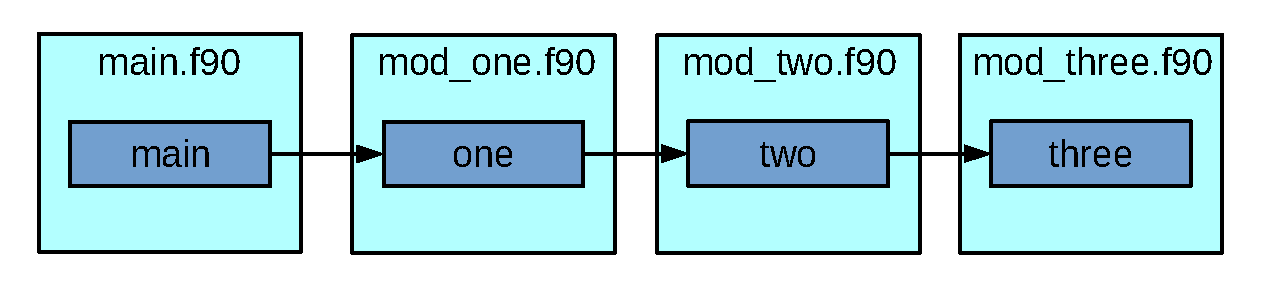
\includegraphics[width=\textwidth]{img/segmentationFault.pdf}  

\end{frame}  


\begin{frame}[fragile,t]
\frametitle{ \huge Another segmentation fault example (ifort)}

\centerline{In which routine the segmentation fault occurs?}

\begin{lstlisting}[language=bash]
$ ./main
forrtl: severe (174): SIGSEGV, segmentation fault occurred
Image              PC                Routine            Line        Source             
main               0000000000469BF9  Unknown               Unknown  Unknown
main               00000000004684CE  Unknown               Unknown  Unknown
main               00000000004379A2  Unknown               Unknown  Unknown
main               000000000041BC98  Unknown               Unknown  Unknown
main               00000000004029FB  Unknown               Unknown  Unknown
libpthread.so.0    00002B86249695E0  Unknown               Unknown  Unknown
main               00000000004026BC  Unknown               Unknown  Unknown
main               0000000000402729  Unknown               Unknown  Unknown
main               000000000040268E  Unknown               Unknown  Unknown
libc.so.6          00002B8624B97C05  Unknown               Unknown  Unknown
main               0000000000402599  Unknown               Unknown  Unknown
\end{lstlisting}

\end{frame}  


\begin{frame}[fragile,t]
\frametitle{ \huge Another segmentation fault example (ifort)}

\centerline{In which routine the segmentation fault occurs?}

\begin{lstlisting}[language=bash]
# Adding "-g -tracback" flags to ifort compiler:
#
$ ./main
forrtl: severe (174): SIGSEGV, segmentation fault occurred
Image              PC                Routine            Line        Source             
...
main               0000000000437A32  Unknown               Unknown  Unknown
main               000000000041BD28  Unknown               Unknown  Unknown
main               0000000000402A8B  Unknown               Unknown  Unknown
libpthread.so.0   00002B3F099255E0  Unknown               Unknown  Unknown
main               00000000004026FC  mod_three_mp_thre    10  mod_three.f90
main               00000000004027EB  mod_two_mp_two_        7  mod_two.f90
main               00000000004027FF  mod_one_mp_one_        7  mod_one.f90
main               00000000004027D2  MAIN__                 4      main.f90
....
\end{lstlisting}

\end{frame} 

\begin{frame}[fragile,t]
\frametitle{ \huge Another segmentation fault example (ifort)}
\begin{lstlisting}[language=fortran,numbers=left]
module mod_three
    implicit none
contains
    subroutine three()
    implicit none
	  INTEGER :: J
	  REAL, ALLOCATABLE :: M (:)

	  DO J=1, 10
		M(J)=4
	  END DO

    end subroutine three
end module mod_three
\end{lstlisting}

\end{frame} 


\subsection{Uninitialized variables} 
\begin{frame}[t]
\frametitle{ Uninitialized variables errors }
\centering
    
\begin{itemize}
  \item An uninitialized variable is a variable that is declared but is its value was not set before it is used.
  \item It will have some value, but not a predictable one.
  \item This can lead to unexpected results and a program failure.
 \end{itemize}

\end{frame}

% \subsection{Uninitialized variable example}
\begin{frame}[fragile,t]
\frametitle{ Uninitialized variable: Example }
\vspace{-10pt}
\begin{lstlisting}[language=fortran,numbers=left]
program compute_factorial
  implicit none 
  integer :: number, i
  write(*,*) 'Type a positive integer number'
  read (*,*) number
  write(*,*) factorial(number)

  contains
  integer function factorial(n)
	integer, intent(in) :: n
	integer :: i
	if (n < 0) error stop 'Only positive integers supported'
	do i = 2, n
	  factorial = factorial * i ! Factorial never initialized!!
	enddo
  end function factorial
end program compute_factorial
\end{lstlisting}

\end{frame}

\begin{frame}[fragile,t]
\frametitle{ Uninitialized variable example: output }
\vspace{-10pt}
\begin{lstlisting}[language=bash]
$ ./compute_factorial 
 Type a positive integer number: 4
 factorial:           0#this is not right...
\end{lstlisting}

\end{frame}



% \subsection{Uninitialized variable debug}
\begin{frame}[fragile,t]
\frametitle{ Uninitialized variable example: debug }

\begin{lstlisting}[language=bash]
$ gfortran  -Wmaybe-uninitialized  -Wuninitialized -O compute_factorial.f90
-o compute_factorial
# These warnings are possible only in optimized compilation!
# Hence, at least -O optimization is needed

compute_factorial.f90: In function ‘compute_factorial’:
compute_factorial.f90:6:0: warning: ‘__result_factorial’ may be 
 used uninitialized in this function [-Wmaybe-uninitialized]
   write(*,*) "factorial:", factorial(number)
 ^
compute_factorial.f90:9:0: note: ‘__result_factorial’ was declared here
   integer function factorial(n)
 ^

\end{lstlisting}


\end{frame}


\begin{frame}[fragile,t]
\frametitle{ Uninitialized variable example: debug }
\vspace{-10pt}
\begin{lstlisting}[language=fortran,numbers=left]
program compute_factorial
  implicit none 
  integer :: number, i
  write(*,*) 'Type a positive integer number'
  read (*,*) number
  write(*,*) factorial(number)

  contains
  integer function factorial(n)
	integer, intent(in) :: n
	integer :: i
	factorial = 1 ! Initialize
	if (n < 0) error stop 'Only positive integers supported'
	do i = 2, n
	  factorial = factorial * i 
	enddo
  end function factorial
end program compute_factorial
\end{lstlisting}

\end{frame}


\begin{frame}[fragile,t]
\frametitle{ Uninitialized variable example: output }
\vspace{-10pt}
\begin{lstlisting}[language=bash]
$ ./compute_factorial 
 Type a positive integer number:
4
 factorial:          24 # Correct!
\end{lstlisting}

\end{frame}


\subsection{Arithmetic errors}
\begin{frame}[t]
\frametitle{Floating points exceptions as a result of a calculation}
\Large
\centering
  \begin{itemize}
   \item \textbf{Invalid}: Invalid operation. E.g. sqrt(-1).
   \item \textbf{Zero division}: Division by zero
   \item \textbf{Overflow}: The result is smaller in absolute value than maximum value that the computer can actually represent.
   \item \textbf{Underflow}: The result is smaller in absolute value than minimum value that the computer can actually represent.
  \end{itemize}
\end{frame}


\begin{frame}[t]
\frametitle{Floating points exception: Example}
\begin{tcolorbox}[colback=mcgillred!5,
  colframe=mcgillred,boxsep=2pt,
  left=0pt,right=0pt,top=5pt,bottom=5pt, title=\textbf{Segmentation fault example}]

  Takes 3 numbers (a,b, and c) and computes a/(b-c) in one of the subroutines.

 \hfill 
 
\dirtree{%
.1 \myfolder{blue}{floating\_point\_exception}.
.2 \myfolder{green}{main.f90}.
.2 \myfolder{green}{mod\_one.f90}.
.2 \myfolder{green}{module\_two.f90}.
.2 \myfolder{green}{module\_three.f90}.
}


\end{tcolorbox}
\end{frame}

 
 \begin{frame}[fragile,t]
\frametitle{ Floating points exception: Example }
\Large
\begin{lstlisting}[language=bash]
$ ./main 
 Type 3 numbers: 5 4 4
 a/(b-c) = Infinity
\end{lstlisting}

\begin{itemize}
 \item Where did this exception happen? 
\end{itemize}

\underline{Debugging}

\begin{itemize}
 \item Add the following compilation flags (gfortran):
 \item \textbf{-g} : Add debug information (important!)
 \item \textbf{-ffpe-trap=underflow,overflow,invalid,zero} : Trap arithmetic errors 
\end{itemize}

\end{frame}


 \begin{frame}[fragile,t]
\frametitle{ Floating points exception: Example }
\Large



\begin{lstlisting}[language=bash]
$ ./main 
 Type 3 numbers: 5 4 4

Program received signal SIGFPE: Floating-point exception 
- erroneous arithmetic operation.

Backtrace for this error:
#0  0x2B86BFC1E6F7
#1  0x2B86BFC1ED3E
#2  0x2B86C06B026F
#3  0x4009AD in __mod_three_MOD_three at mod_three.f90:9 #Here!!
#4  0x400BC7 in __mod_two_MOD_two at mod_two.f90:9
#5  0x400BF9 in __mod_one_MOD_one at mod_one.f90:10
#6  0x400AD5 in MAIN__ at main.f90:7
Floating point exception (core dumped)
\end{lstlisting}
\end{frame}


\begin{frame}[fragile,t]
\frametitle{ Floating points exception: Example }
\vspace{-10pt}
\begin{lstlisting}[language=fortran,numbers=left]
module mod_three
    implicit none
contains
    subroutine three(a,b,c,d)
    implicit none
	  REAL,INTENT(IN) :: a,b,c
	  REAL,INTENT(OUT) :: d
	  
	  d = a/(b-c)

    end subroutine three
end module mod_three
\end{lstlisting}

\end{frame}
%http://earth.uni-muenster.de/~joergs/doc/f90/unix-um/dfum_034.html


\begin{frame}[t]
\frametitle{ More on Floating-point arithmetic
\footnote{http://jules-lsm.github.io/coding\_standards/guidelines/fp\_arithmetic.html}}
\Large

\begin{itemize}
 \item Due to the limited precision available to represent real numbers, things that are true for normal arithmetic no longer hold in floating-point arithmetic.
\end{itemize}

\end{frame}

\begin{frame}[fragile,t]
\frametitle{ More on Floating-point arithmetic
\footnote{http://jules-lsm.github.io/coding\_standards/guidelines/fp\_arithmetic.html}}
\Large

\begin{itemize}
 \item Comparing 2 float numbers
\end{itemize}

\begin{lstlisting}[language=fortran,numbers=left]
IF ( precipitation(x,y) > 0.0 ) THEN
  ! Do something
ELSE
  ! Do something else
END IF
\end{lstlisting}


\begin{itemize}
 \item Due to rounding errors or optimizations, in places were we expect to have zero precipitation a very low value can be encountered. 
 \end{itemize}

\end{frame}

\begin{frame}[fragile,t]
\frametitle{ More on Floating-point arithmetic
\footnote{http://jules-lsm.github.io/coding\_standards/guidelines/fp\_arithmetic.html}}
\large

\begin{itemize}
  \item Due to rounding errors or optimizations, in places were we expect to have zero precipitation a very low value can be encountered. 
 \item \textbf{Solution}: specify a physically realistic tolerance level.
\end{itemize}

\begin{lstlisting}[language=fortran,numbers=left]
IF ( precipitation(x,y) > tolerance ) THEN
  ! Do something
ELSE
  ! Do something else
END IF
\end{lstlisting}

\end{frame}


\begin{frame}[fragile,t]
\frametitle{ More on Floating-point arithmetic
\footnote{http://jules-lsm.github.io/coding\_standards/guidelines/fp\_arithmetic.html}}
\large

\begin{itemize}
  \item More about rounding errors 
\end{itemize}

\begin{lstlisting}[language=fortran,numbers=left]
IF ( a_real_number == other_real_number ) THEN
  ! Do something
ELSE
  ! Do something else
END IF

!!! Better approach
IF ( ABS(a_real_number – other_real_number) < tolerance ) THEN
  ! Do something
ELSE
  ! Do something else
END IF
\end{lstlisting}

\end{frame}


\section{Logical errors} 

\begin{frame}[t]
\frametitle{ \huge Logical errors}
  \Large
  \setbeamercovered{transparent}
  \begin{tightBox}
  \centering 
  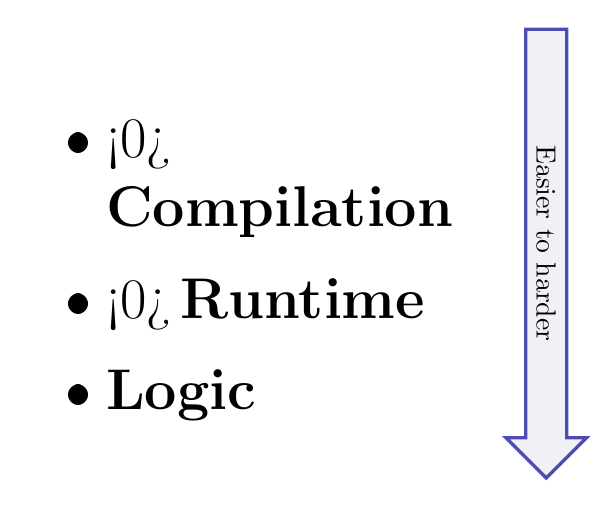
\begin{tikzpicture}[node distance=0pt,
		      SA/.style = {single arrow, draw=blue!40!gray, very thick, fill=blue!20!gray!10,
		      minimum height=1.2*\n1} ]
		      
   \node (n)   [text width=0.5\textwidth]
{
  \huge
      \begin{itemize}	
	\item<0> \textbf{Compilation}
	\item<0> \textbf{Runtime}
	\item \textbf{Logic}
      \end{itemize}           
};
\path   let \p1 = ($(n.north)-(n.south)$),
            \n1 = {veclen(\y1,\x1)} in
        node[SA, rotate=-90,  xshift=-\n1/2,
             above=of n.south east] {Easier to harder};
\end{tikzpicture}
  \end{tightBox}
 
\end{frame} 


 \begin{frame}[t]
  \frametitle{ Logical errors }
  \begin{itemize}
    \item The program appears to run correctly, by it gives wrong or unexpected results.
    \item One approach to solve them is to test different parts of the program with inputs with known outputs.
  \end{itemize}

  \centering
  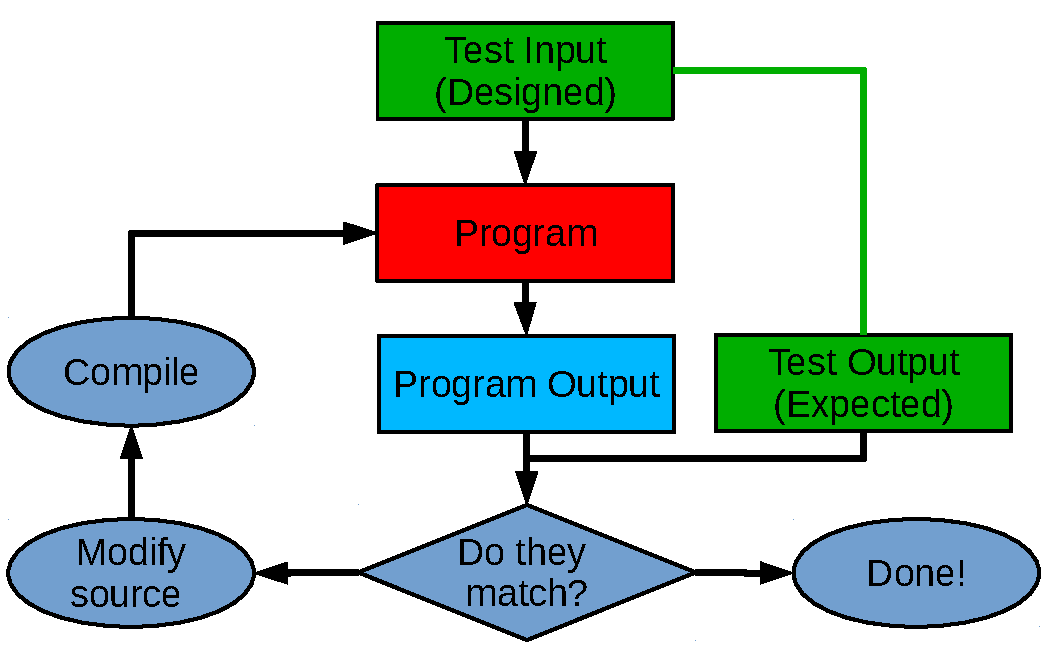
\includegraphics[width=0.75\textwidth]{img/testing.pdf} 
\end{frame} 


\section{Final remarks}
\begin{frame}[t]
  \frametitle{ \huge Final remarks }
  \centering
   \Large
\only<+>{
  \begin{itemize}
    \item{First fix all the compilation errors and warnings
     \large
    \begin{itemize}
      \item Compile and run the program with the following flags (gfortran):
      \item \textbf{-fcheck=bounds}
      \item \textbf{-Wmaybe-uninitialized  -Wuninitialized -O}       
    \end{itemize}
    }
  \end{itemize}
}

\only<+>{
    \begin{itemize}
    \item{If an error is detected on runtime:
    
    \begin{itemize}
      \large
      \item Recompile and run the program with the following flags (gfortran):
      \item \textbf{-fcheck=bounds} (check arrays bounds)
      \item \textbf{-O0}  ( disable optimizations!)
      \item \textbf{-g -fbacktrace} (add debugging information!)
      \item \textbf{-ffpe-trap=underflow,overflow,invalid,zero} (trap floating point exceptions)
    \end{itemize}
    }
  \end{itemize}
}

\only<+>{
    \begin{itemize}
    \item{Run test cases to find logical errors }
    \end{itemize}
    
    \centering
    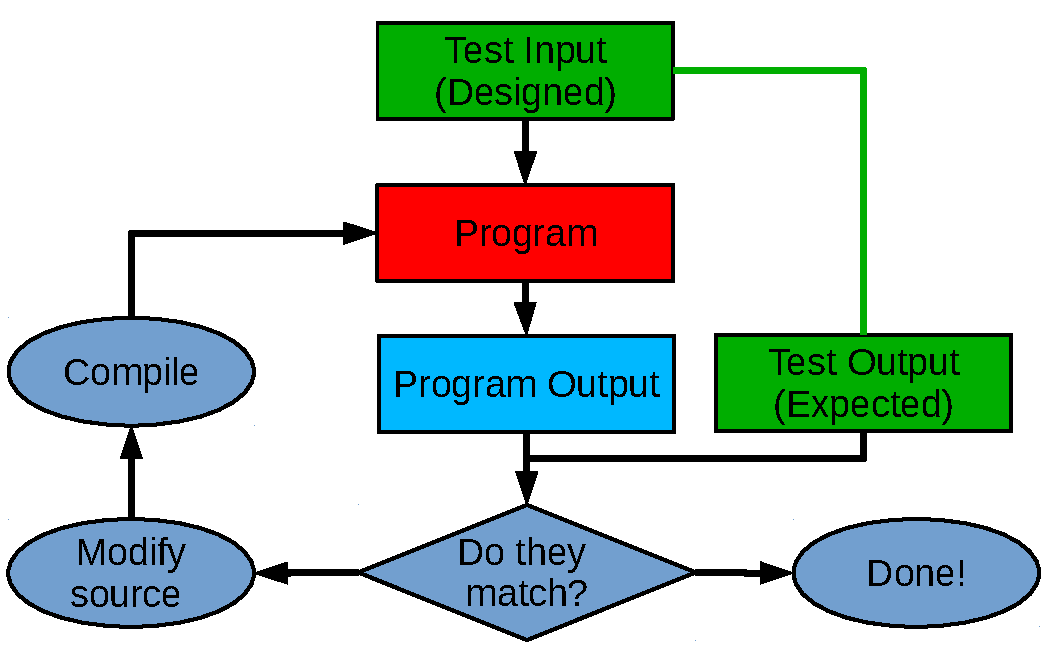
\includegraphics[width=0.75\textwidth]{img/testing.pdf} 
}


\end{frame}

% % Float equal comparison
% % http://jules-lsm.github.io/coding_standards/guidelines/fp_arithmetic.html
% \begin{frame}[t]
% \frametitle{ More resources }
% \centering
%     
% \begin{itemize}
%  \item Introduction to debugging:
%     \begin{itemize}
%     \item \url{https://vimeo.com/channels/debugging/}
%     \item{\url{https://gcc.gnu.org/onlinedocs/gcc-4.0.2/gcc/Warning-Options.html}  }
%     \end{itemize}
% \end{itemize}
% 
% \end{frame}



% \section{Tips} 
% 
% https://github.com/cogrhythms/good-coding-practices/wiki
% https://software-carpentry.org/blog/2012/10/best-practices-for-scientific-computing.html
% 


\end{document}


